\documentclass[tikz,border=10pt]{standalone}
\usetikzlibrary{arrows.meta, positioning, shapes.geometric, shapes.misc, fit, backgrounds, calc, matrix}

\tikzset{
    >=Latex,
    font=\sffamily\large,
    node distance=1.5cm and 3cm,
    dag_result/.style={
        rectangle, 
        draw=green!70!black, 
        fill=green!15, 
        very thick, 
        minimum width=4.5cm, 
        minimum height=1.5cm, 
        text width=5cm,
        align=center
    },
    dag_lemma/.style={
        rounded rectangle, 
        draw=orange!80!black, 
        fill=yellow!20, 
        very thick, 
        minimum width=4.5cm, 
        minimum height=1.5cm, 
        text width=5cm,
        align=center
    },
    dag_model/.style={
        ellipse, 
        draw=blue!70!black, 
        fill=blue!12, 
        very thick, 
        minimum width=4.5cm, 
        minimum height=1.5cm, 
        text width=4.5cm,
        align=center
    },
    dag_unformalized/.style={
        rectangle, 
        draw=gray!60!black, 
        fill=gray!10, 
        very thick, 
        dashed, 
        minimum width=4.5cm, 
        minimum height=1.5cm, 
        text width=5cm,
        align=center
    },
    dag_conditional/.style={
        rectangle, 
        rounded corners,
        draw=orange!80!black, 
        fill=orange!10, 
        very thick, 
        minimum width=4.5cm, 
        minimum height=1.5cm, 
        text width=5cm,
        align=center
    },
    dag_partial/.style={
        rectangle,
        rounded corners,
        draw=yellow!55!black,
        fill=yellow!10,
        very thick,
        dashed,
        minimum width=4.5cm,
        minimum height=1.5cm,
        text width=5cm,
        align=center
    },
    dag_scaffold/.style={
        rectangle,
        draw=gray!55!black,
        fill=white,
        very thick,
        dotted,
        minimum width=4.5cm,
        minimum height=1.5cm,
        text width=5cm,
        align=center
    },
    dag_caveat/.style={
        diamond, 
        draw=red!70!black, 
        fill=red!10, 
        minimum width=4cm, 
        align=center, 
        inner sep=0pt, 
        font=\sffamily\small
    },
    dag_arrow/.style={
        -{Stealth[scale=1.2]}, 
        very thick,
        shorten >=1.5pt,
        shorten <=1.5pt
    },
    dag_dashed_arrow/.style={
        -{Stealth[scale=1.2]}, 
        very thick, 
        dashed,
        shorten >=1.5pt,
        shorten <=1.5pt
    },
    dag_template_legend/.style={
        minimum width=2.6cm,
        minimum height=0.8cm,
        text width=2.45cm,
        inner sep=3pt,
        font=\sffamily\small,
        align=center
    },
    dag_template_note/.style={
        rectangle,
        draw=gray!50,
        fill=gray!5,
        rounded corners,
        text width=13cm,
        align=left,
        font=\sffamily\small,
        inner sep=6pt
    }
}

% Legend Helper
\newcommand{\daglegend}[2]{
    \node[draw, rounded corners, very thick, fit=#1, inner sep=12pt, label=above:\textbf{\Large Legend}] (#2) {};
}


\begin{document}
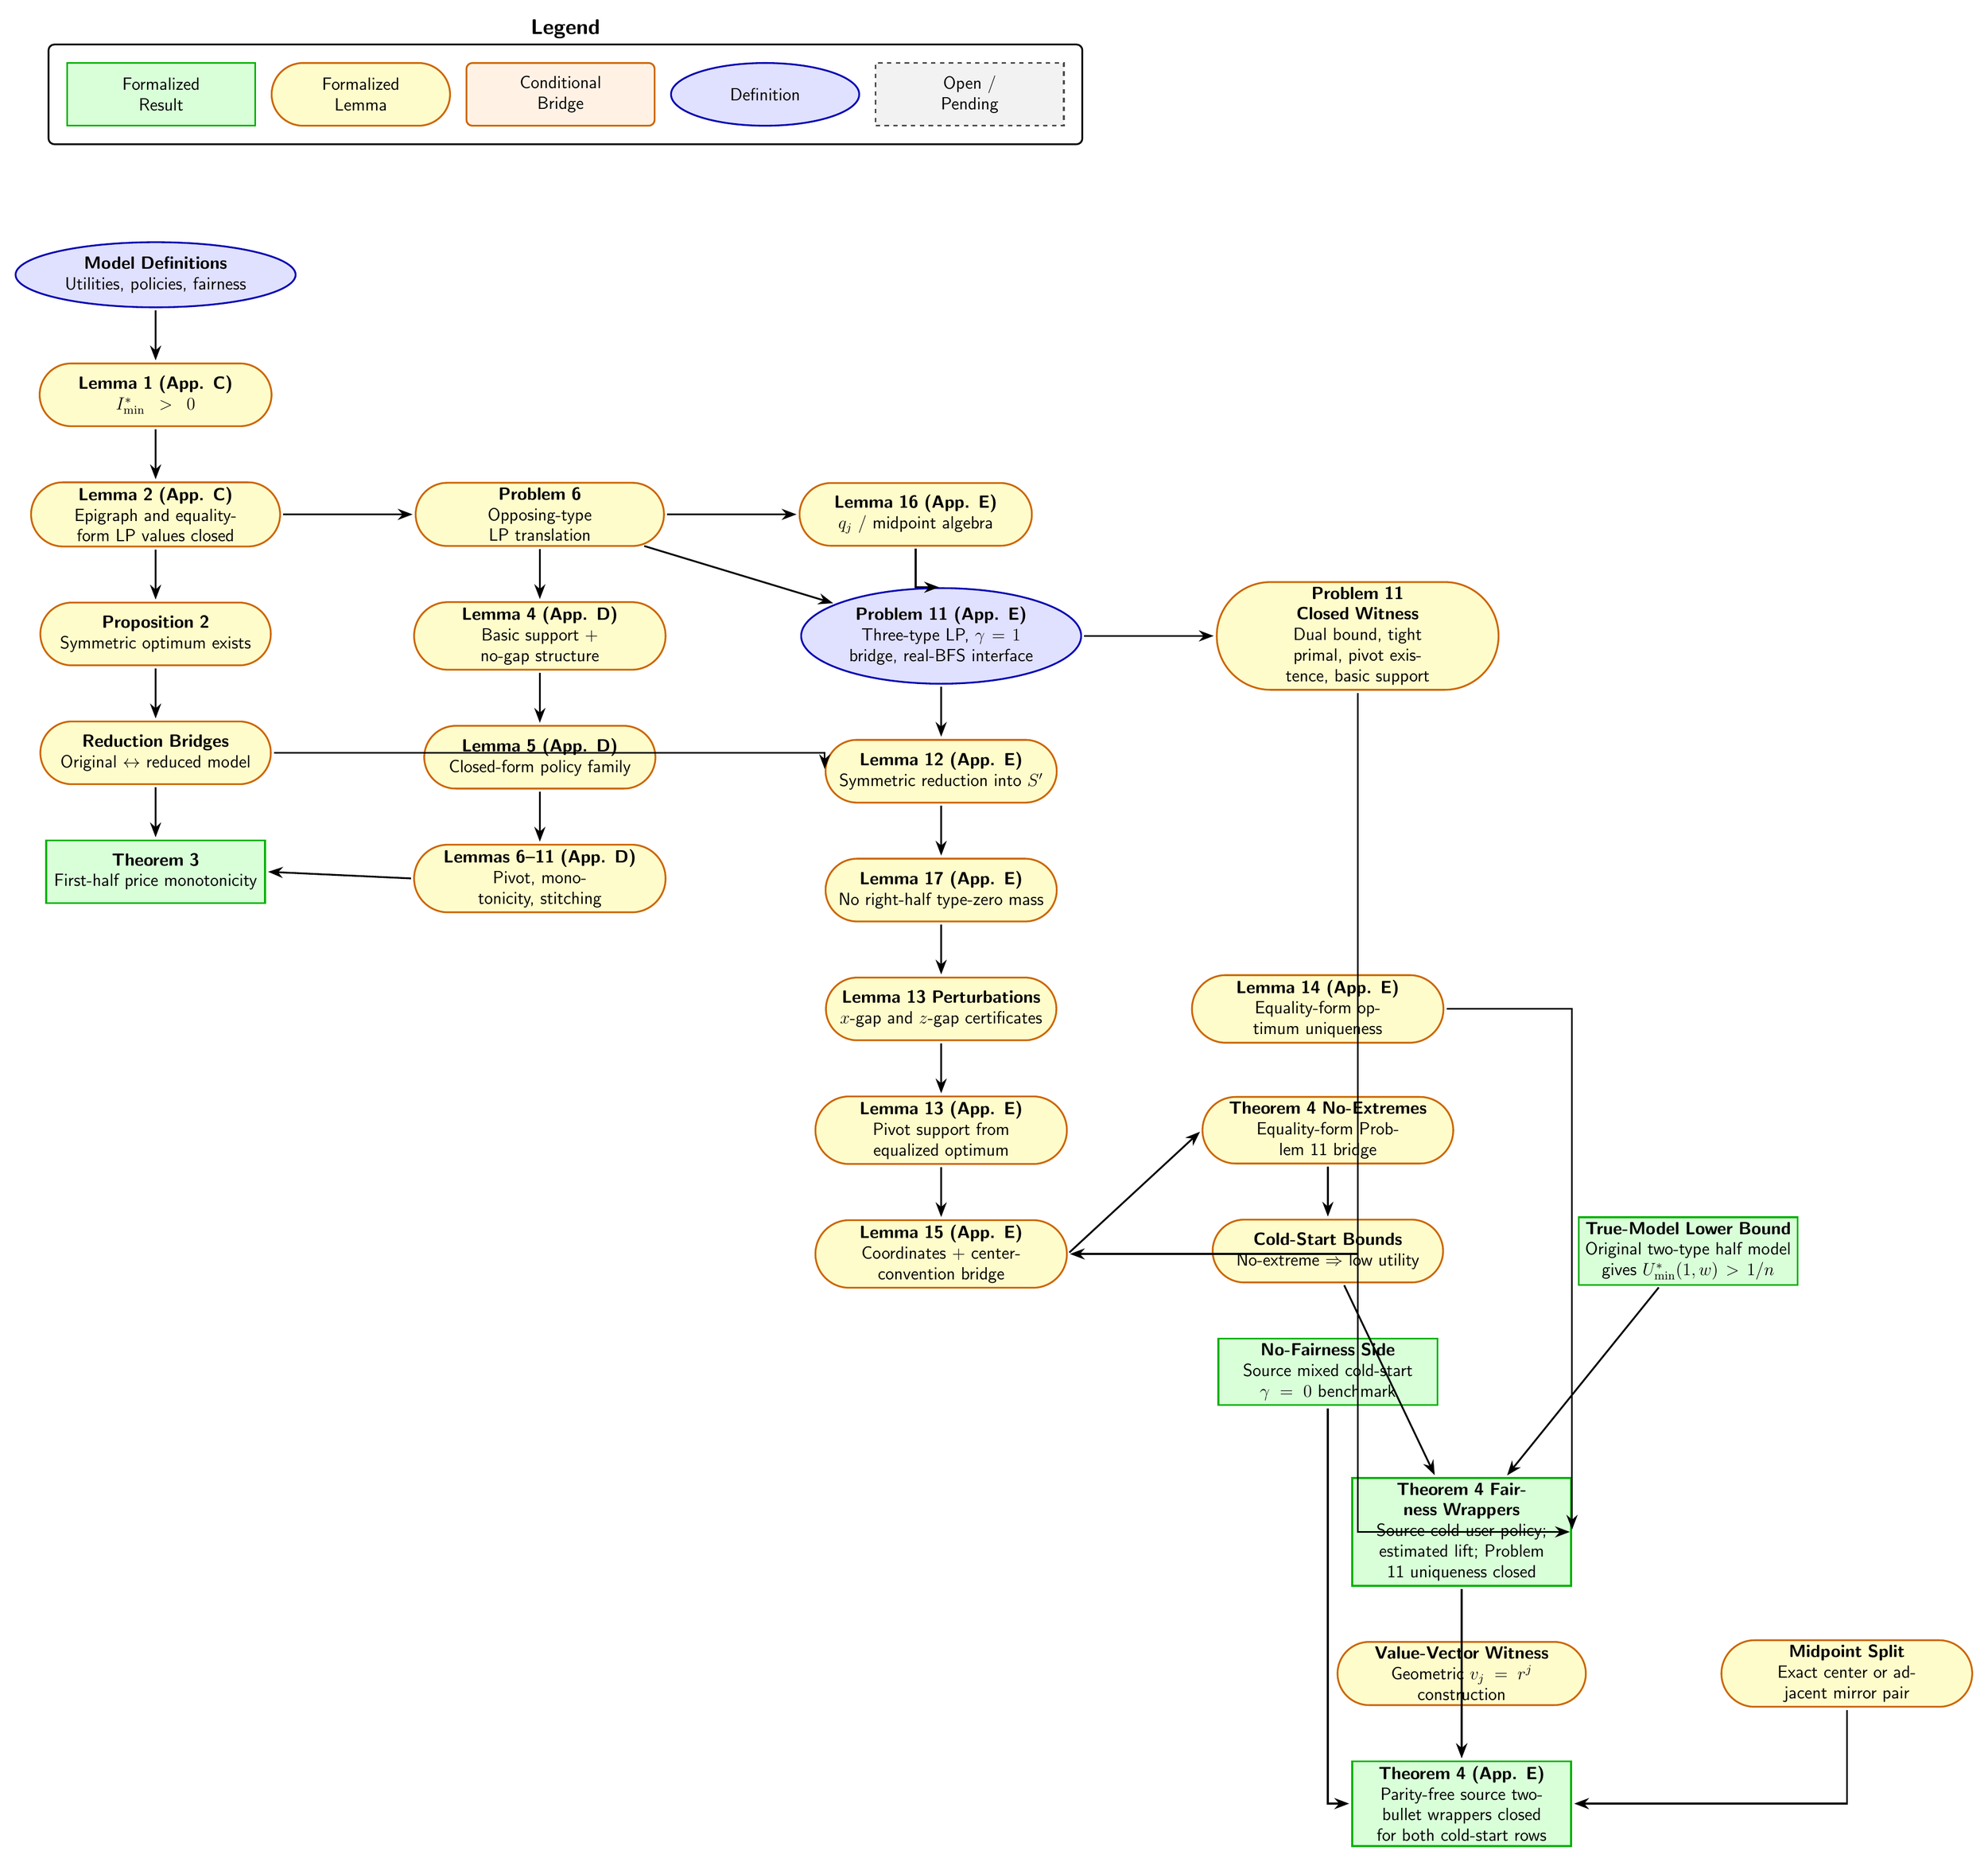
\begin{tikzpicture}[node distance=1.3cm and 3.2cm]

% --- Legend ---
\node[dag_result, text width=2.6cm] (legRes) {Formalized Result};
\node[dag_lemma, right=0.35cm of legRes, text width=2.6cm] (legLem) {Formalized Lemma};
\node[dag_conditional, right=0.35cm of legLem, text width=2.8cm] (legCond) {Conditional Bridge};
\node[dag_model, right=0.35cm of legCond, text width=2.5cm] (legDef) {Definition};
\node[dag_unformalized, right=0.35cm of legDef, text width=2.7cm] (legOpen) {Open / Pending};
\daglegend{(legRes)(legLem)(legCond)(legDef)(legOpen)}{Legend}

% --- Core model, reduction, and Theorem 3 ---
\node[dag_model, below=2.3cm of Legend, xshift=-9.8cm] (BaseDefs)
  {\textbf{Model Definitions} \\ Utilities, policies, fairness};
\node[dag_lemma, below=of BaseDefs] (Lemma1)
  {\textbf{Lemma 1 (App. C)} \\ $I^*_{\min} > 0$};
\node[dag_lemma, below=of Lemma1] (Lemma2)
  {\textbf{Lemma 2 (App. C)} \\ Epigraph and equality-form LP values closed};
\node[dag_lemma, below=of Lemma2] (Prop2)
  {\textbf{Proposition 2} \\ Symmetric optimum exists};
\node[dag_lemma, below=of Prop2] (Reduction)
  {\textbf{Reduction Bridges} \\ Original $\leftrightarrow$ reduced model};
\node[dag_result, below=of Reduction] (Theorem3)
  {\textbf{Theorem 3} \\ First-half price monotonicity};

% --- Problem 6 / Appendix D structure ---
\node[dag_lemma, right=of Lemma2] (Problem6)
  {\textbf{Problem 6} \\ Opposing-type LP translation};
\node[dag_lemma, below=of Problem6] (Lemma4)
  {\textbf{Lemma 4 (App. D)} \\ Basic support + no-gap structure};
\node[dag_lemma, below=of Lemma4] (Lemma5)
  {\textbf{Lemma 5 (App. D)} \\ Closed-form policy family};
\node[dag_lemma, below=of Lemma5] (Lemmas6to11)
  {\textbf{Lemmas 6--11 (App. D)} \\ Pivot, monotonicity, stitching};
\node[dag_lemma, right=of Problem6] (Lemma16)
  {\textbf{Lemma 16 (App. E)} \\ $q_j$ / midpoint algebra};

% --- Problem 11 and Theorem 4 support structure ---
\node[dag_model, right=of Lemma4] (Problem11)
  {\textbf{Problem 11 (App. E)} \\ Three-type LP, $\gamma=1$ bridge, real-BFS interface};
\node[dag_lemma, right=of Problem11] (Problem11Dual)
  {\textbf{Problem 11 Closed Witness} \\ Dual bound, tight primal, pivot existence, basic support};
\node[dag_lemma, below=of Problem11] (Lemma12)
  {\textbf{Lemma 12 (App. E)} \\ Symmetric reduction into $S'$};
\node[dag_lemma, below=of Lemma12] (Lemma17)
  {\textbf{Lemma 17 (App. E)} \\ No right-half type-zero mass};
\node[dag_lemma, below=of Lemma17] (NoGap)
  {\textbf{Lemma 13 Perturbations} \\ $x$-gap and $z$-gap certificates};
\node[dag_lemma, below=of NoGap] (Lemma13)
  {\textbf{Lemma 13 (App. E)} \\ Pivot support from equalized optimum};
\node[dag_lemma, below=of Lemma13] (Lemma15)
  {\textbf{Lemma 15 (App. E)} \\ Coordinates + center-convention bridge};

% --- Theorem 4 downstream wrappers and open paper theorem ---
\node[dag_lemma, right=of NoGap] (Lemma14)
  {\textbf{Lemma 14 (App. E)} \\ Equality-form optimum uniqueness};
\node[dag_lemma, right=of Lemma13] (NoExtremes)
  {\textbf{Theorem 4 No-Extremes} \\ Equality-form Problem 11 bridge};
\node[dag_lemma, below=of NoExtremes] (ColdBounds)
  {\textbf{Cold-Start Bounds} \\ No-extreme $\Rightarrow$ low utility};
\node[dag_result, below=of ColdBounds] (NoFairness)
  {\textbf{No-Fairness Side} \\ Source mixed cold-start $\gamma=0$ benchmark};
\node[dag_result, right=of ColdBounds] (TrueLower)
  {\textbf{True-Model Lower Bound} \\ Original two-type half model gives $U^*_{\min}(1,w) > 1/n$};
\node[dag_result, below=1.7cm of NoFairness, xshift=3.2cm] (Theorem4Conditional)
  {\textbf{Theorem 4 Fairness Wrappers} \\ Source cold-user policy; estimated lift; Problem 11 uniqueness closed};
\node[dag_lemma, below=of Theorem4Conditional] (VExist)
  {\textbf{Value-Vector Witness} \\ Geometric $v_j=r^j$ construction};
\node[dag_lemma, right=of VExist] (Midpoint)
  {\textbf{Midpoint Split} \\ Exact center or adjacent mirror pair};
\node[dag_result, below=of VExist] (Theorem4Full)
  {\textbf{Theorem 4 (App. E)} \\ Parity-free source two-bullet wrappers closed for both cold-start rows};

% --- Edges: model/reduction path ---
\draw[dag_arrow] (BaseDefs) -- (Lemma1);
\draw[dag_arrow] (Lemma1) -- (Lemma2);
\draw[dag_arrow] (Lemma2) -- (Prop2);
\draw[dag_arrow] (Prop2) -- (Reduction);
\draw[dag_arrow] (Reduction) -- (Theorem3);

% --- Edges: Problem 6 / Theorem 3 path ---
\draw[dag_arrow] (Lemma2) -- (Problem6);
\draw[dag_arrow] (Problem6) -- (Lemma4);
\draw[dag_arrow] (Lemma4) -- (Lemma5);
\draw[dag_arrow] (Lemma5) -- (Lemmas6to11);
\draw[dag_arrow] (Lemmas6to11.west) -- (Theorem3.east);
\draw[dag_arrow] (Problem6) -- (Lemma16);

% --- Edges: Problem 11 / Lemma 13 path ---
\draw[dag_arrow] (Problem6) -- (Problem11);
\draw[dag_arrow] (Lemma16.south) |- (Problem11.north);
\draw[dag_arrow] (Reduction.east) -| (Lemma12.west);
\draw[dag_arrow] (Problem11) -- (Lemma12);
\draw[dag_arrow] (Problem11) -- (Problem11Dual);
\draw[dag_arrow] (Problem11Dual.south) |- (Lemma15.east);
\draw[dag_arrow] (Lemma12) -- (Lemma17);
\draw[dag_arrow] (Lemma17) -- (NoGap);
\draw[dag_arrow] (NoGap) -- (Lemma13);
\draw[dag_arrow] (Lemma13) -- (Lemma15);
\draw[dag_arrow] (Lemma15.east) -- (NoExtremes.west);

% --- Edges: Theorem 4 path ---
\draw[dag_arrow] (NoExtremes) -- (ColdBounds);
\draw[dag_arrow] (ColdBounds) -- (Theorem4Conditional);
\draw[dag_arrow] (NoFairness) |- (Theorem4Full.west);
\draw[dag_arrow] (TrueLower) -- (Theorem4Conditional);
\draw[dag_arrow] (Problem11Dual.south) |- (Theorem4Conditional.east);
\draw[dag_arrow] (Lemma14.east) -| (Theorem4Conditional.east);
\draw[dag_arrow] (Theorem4Conditional) -- (Theorem4Full);
\draw[dag_arrow] (VExist) -- (Theorem4Full);
\draw[dag_arrow] (Midpoint) |- (Theorem4Full);

\end{tikzpicture}
\end{document}
